\documentclass[10pt]{scrartcl}

\usepackage[utf8]{inputenc}
\usepackage{tabularx}
\usepackage[ngerman]{babel}
\usepackage[automark]{scrpage2}
\usepackage{amsmath,amssymb,amstext}
%\usepackage{mathtools}

\usepackage[]{enumerate}
\usepackage{graphicx}
\usepackage{lastpage}
\usepackage[perpage,para,symbol*]{footmisc}
\usepackage{listings}
\usepackage{color}
\usepackage{textcomp}
\definecolor{listinggray}{gray}{0.9}
\definecolor{lbcolor}{rgb}{0.9,0.9,0.9}
\lstset{
	backgroundcolor=\color{lbcolor},
	tabsize=4,
	rulecolor=,
	language=matlab,
        basicstyle=\scriptsize,
        upquote=true,
        aboveskip={1.5\baselineskip},
        columns=fixed,
        showstringspaces=false,
        extendedchars=true,
        breaklines=true,
        prebreak = \raisebox{0ex}[0ex][0ex]{\ensuremath{\hookleftarrow}},
        frame=single,
        showtabs=false,
        showspaces=false,
        showstringspaces=false,
        identifierstyle=\ttfamily,
        keywordstyle=\color[rgb]{0,0,1},
        commentstyle=\color[rgb]{0.133,0.545,0.133},
        stringstyle=\color[rgb]{0.627,0.126,0.941},
}
\usepackage[pdfborder={0 0 0},colorlinks=false]{hyperref}
\usepackage[numbers,square]{natbib}
\usepackage{float}

\lstset{numbers=left, numberstyle=\tiny, numbersep=5pt, breaklines=true, showstringspaces=false} 

%changehere
\def\titletext{Praktikum 1 : DGL}
\def\titletextshort{Praktikum 1}
\author{Oliver Steenbuck, Karolina Bernat}

\title{\titletext}

%changehere Datum der Übung
\date{31.10.2012}

\pagestyle{scrheadings}
%changehere
\ihead{MT, Pareigis}
\ifoot{Generiert am:\\ \today}

\cfoot{Karolina Bernat, Oliver Steenbuck}


\ohead[]{\titletextshort}
\ofoot[]{{\thepage} / \pageref{LastPage}}

\setlength{\parindent}{0.0in}
\setlength{\parskip}{0.1in}

\begin{document}
\maketitle
\setcounter{tocdepth}{3}
\tableofcontents
\listoffigures
\lstlistoflistings


\section{Steife Differentialgleichungen}
Gegeben ist folgende Differentialgleichung 1. Grades an der mit Matlab und Simulink drei verschiedene Approximationsverfahren (Explizites und implizites Euler Verfahren sowie das Verfahren von Runge Kutta 2. Ordnung) für steife Differentialgleichungen angewendet werden sollen.
\subsection{Gleichung} \label{aufg1Gleich}
	\begin{align}
		&y(0)=1\\
		&y'=10-500 \cdot y + 5000 \cdot x
	\end{align}
	
	
	\subsection{Simulink}
	Die in \ref{aufg1Gleich} gezeigte Gleichung wurde zuerst in Simulink modelliert.
		\begin{figure}[H]
			\centering	
			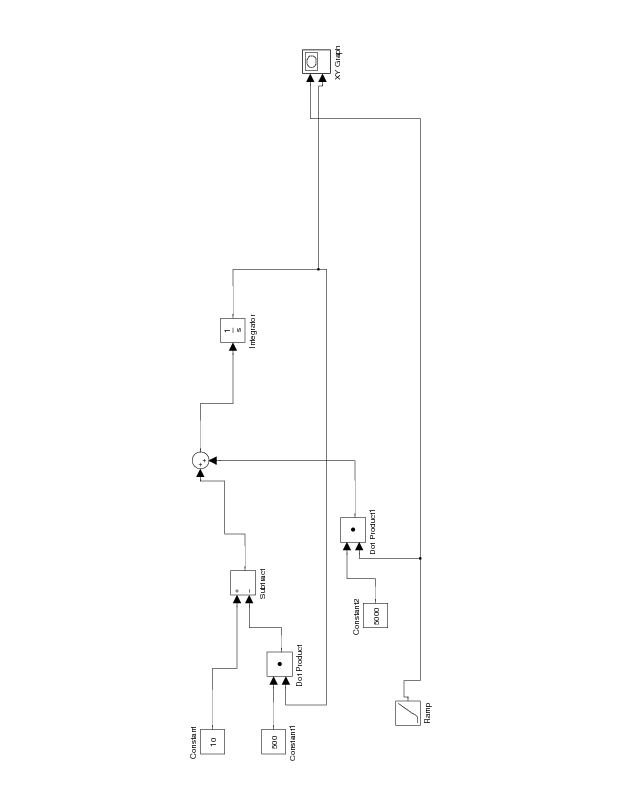
\includegraphics[width=\textwidth, angle=-90]{Prak1Aufg1Simulink.png}
            \caption{Steife Differentialgleichung Simulink}
            \label{pic:lorenzSimulink}
		\end{figure} 	
	
	\subsection{Iterationslgeichungen}	
	Untenstehend wurden die für die jeweiligen Verfahren notwendigen Iterationsgleichungen hergeleitet und die Verfahren in Matlab implementiert, siehe \ref{sec:matlab}.
	\subsubsection{Euler, explizit}
	Eingesetzt in das explizite Euler Verfahren ergibt sich folgende Iterationsgleichung.
	\begin{align}
		&y(0)=1\\
		&y_{j+1}=y_{j} + h \cdot (10-500 \cdot y_{j} + 5000 \cdot x_j)
	\end{align}
	
	\subsubsection{Euler, implizit}
	Für das implizite Euler Verfahren ergibt sich die nachstehende Gleichung, wobei hier $y_{j+1}$ mit dem Newton oder einem anderen Verfahren zur Nullstellenberechnung approximiert werden muß.
	\begin{align}
		&y(0)=1\\
		&y_{j+1}=y_{j} + h \cdot (10-500 \cdot y_{j+1} + 5000 \cdot x_{j+1})
	\end{align}
	
	
	\subsubsection{Runge Kutta 2. Ordnung}
	Zur Vereinfachung der Iterationsgleichung im Runge Kutta 2 Verfahren gelte  (\ref{vereinfach})
	\begin{align}	
	 f(x) = 10-500 \cdot y + 5000 \cdot x \label{vereinfach} 
	\end{align}
	Dann ergibt sich durch einsetzen in die Runge Kutta Gleichung.
	\begin{align}
		&y(0)=1\\
		&y_{j+1}=y_{j} + \frac{h}{2} \cdot (f(x_{j+1}, y_{j}) + f(x_{j+1}, h \cdot f(x_j, y_j)) )
	\end{align}

\subsection{Matlab Programme}
	\lstinputlisting[tabsize=2, frame=single, label=Stiff, caption={Stiff}]{stiff.m}
	\lstinputlisting[tabsize=2, frame=single, label=steifeDiff, caption={Steife Differentialgleichung}]{f.m}

\subsection{Ergebnisse}
	Im folgenden sind die Approximationen durch alle 3 Verfahren mit Schrittweiten von ($0.001$ bis $0.005$) grapthisch dargestellt. Deutlich erkennbar wird hier wie die expliziten Verfahren (Expliziter Euler, Runge Kutta 2. Ordnung) gegenüber dem impliziten Euler Verfahren bei wachsender Schrittweite an Genauigkeit verlieren, wie dies auch zu erwarten war.

		\begin{figure}[H]
			\centering	
			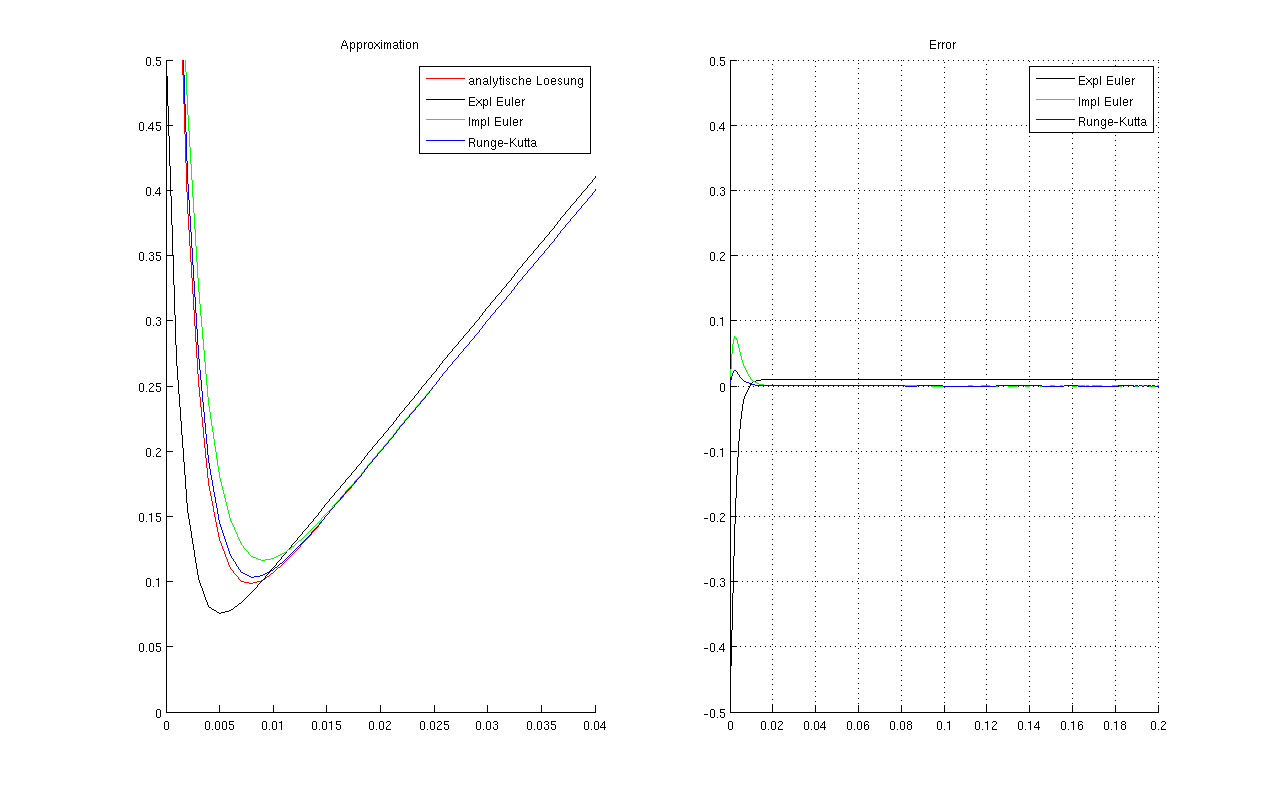
\includegraphics[width=\textwidth]{stiff0001.png}
            \caption{Stiff (h=0.001)}
            \label{pic:stuff001}
		\end{figure} 
	
	
	\begin{figure}[H]
			\centering	
			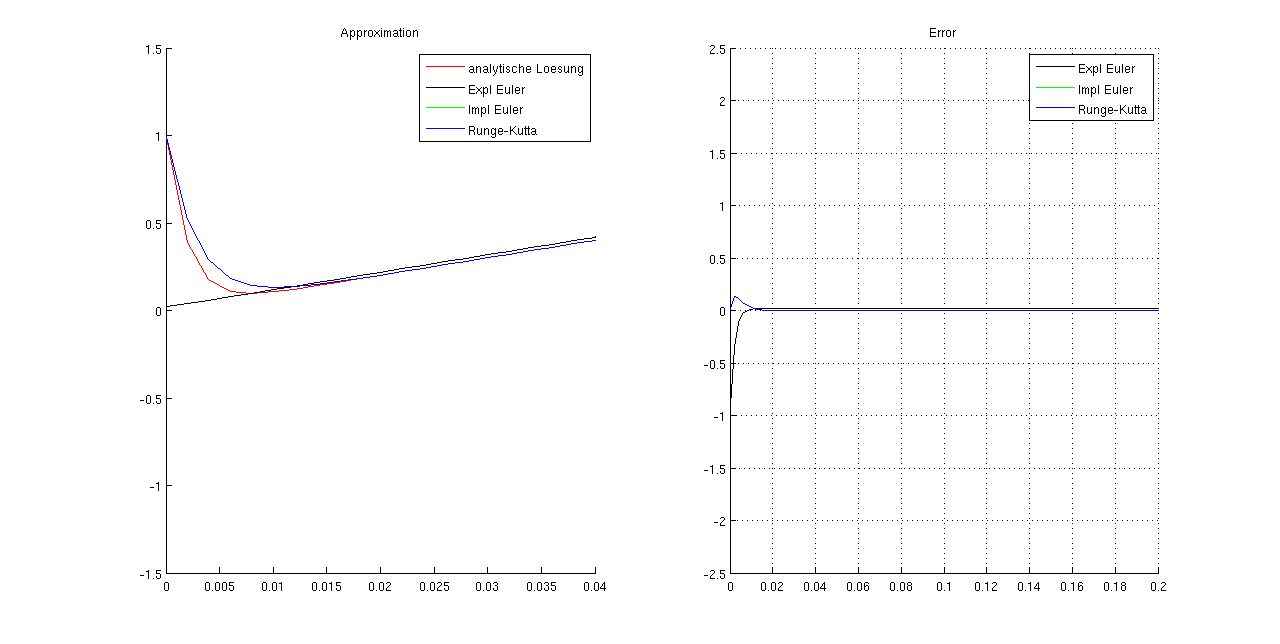
\includegraphics[width=\textwidth]{stiff0002.png}
            \caption{Stiff (h=0.002)}
            \label{pic:stuff002}
		\end{figure} 
	
	
	\begin{figure}[H]
			\centering	
			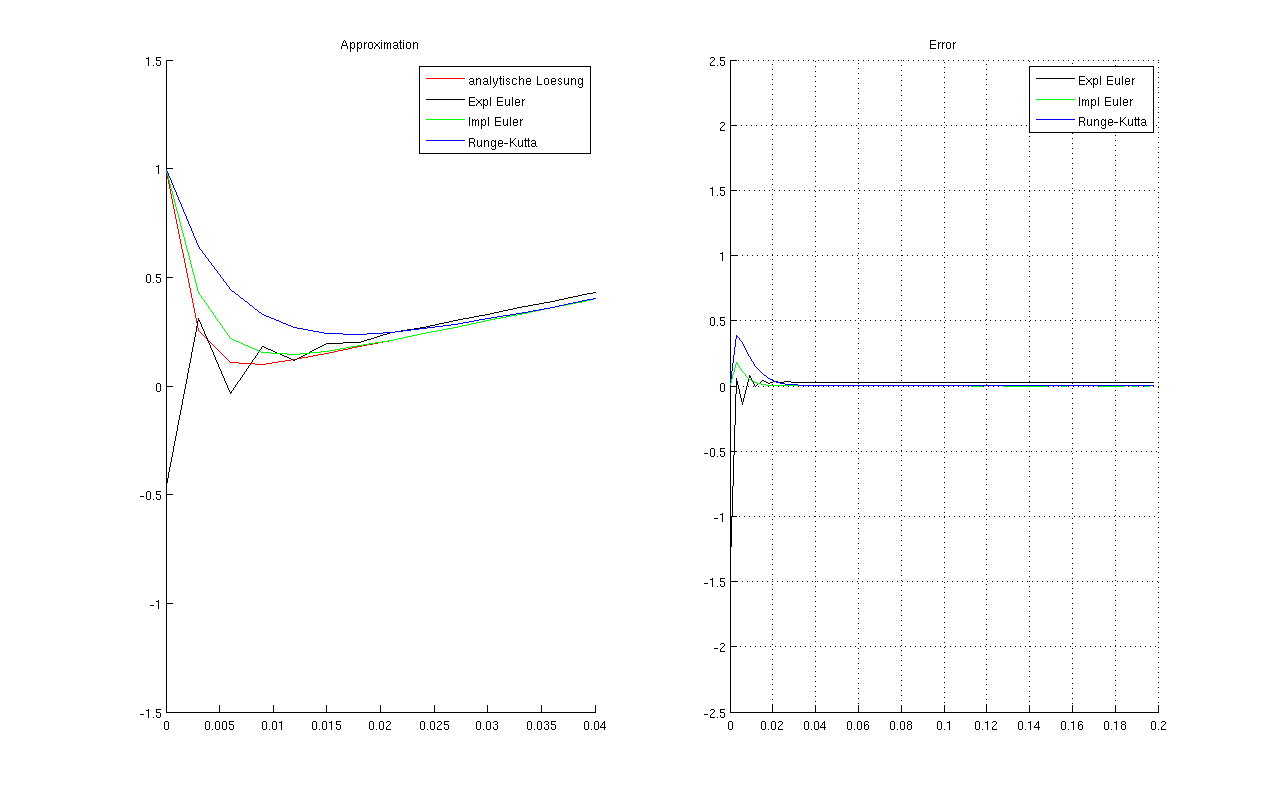
\includegraphics[width=\textwidth]{stiff0003.png}
            \caption{Stiff (h=0.003)}
            \label{pic:stuff003}
		\end{figure} 
	
	
	\begin{figure}[H]
			\centering	
			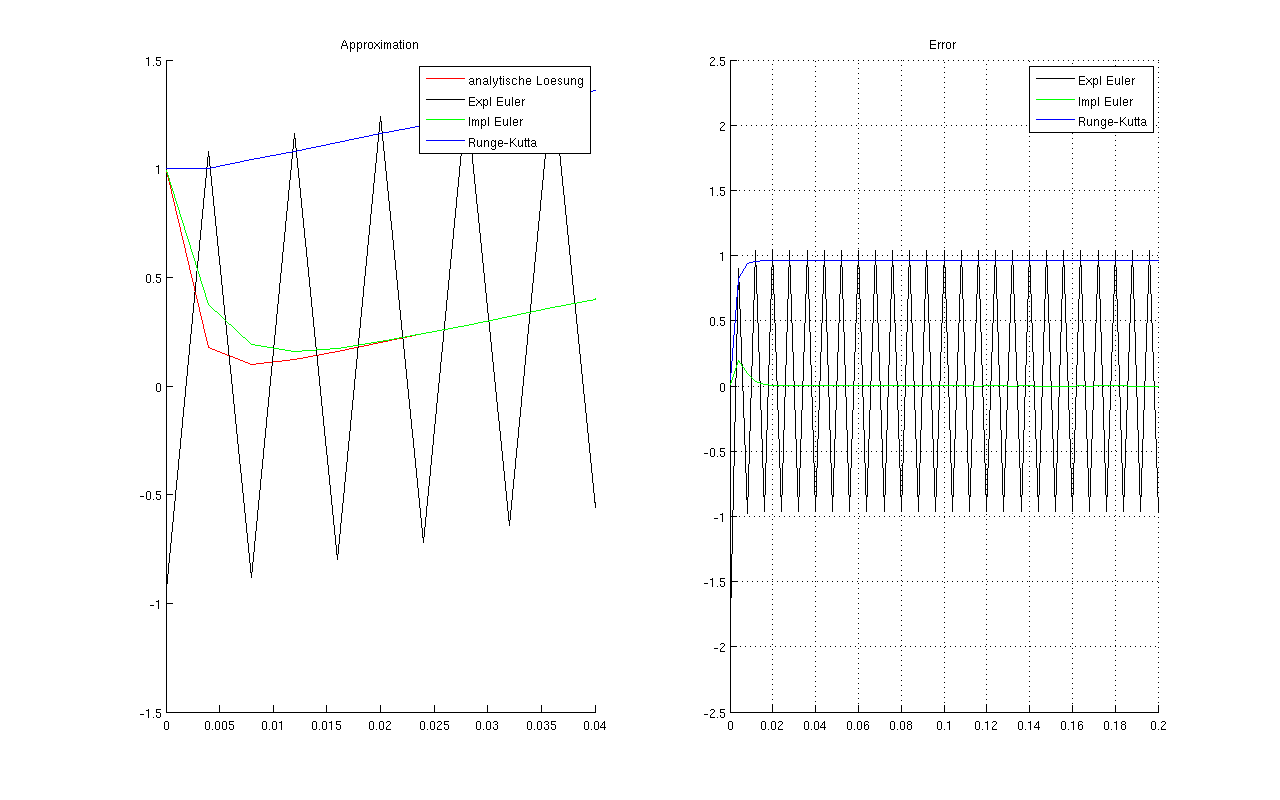
\includegraphics[width=\textwidth]{stiff0004.png}
            \caption{Stiff (h=0.004)}
            \label{pic:stuff004}
		\end{figure} 
	
	\begin{figure}[H]
			\centering	
			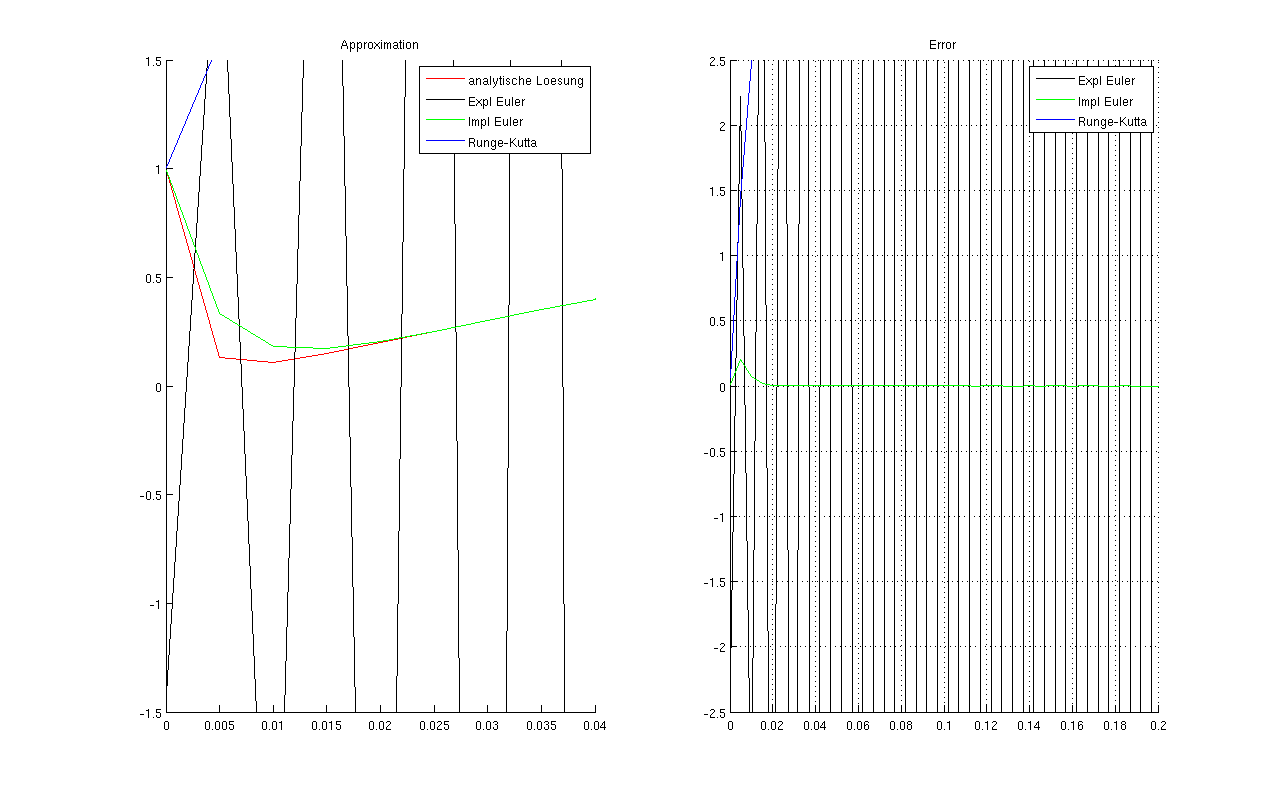
\includegraphics[width=\textwidth]{stiff0005.png}
            \caption{Stiff (h=0.005)}
            \label{pic:stuff005}
		\end{figure} 

\section{Van der Pol DGL}
	\subsection{Gleichung}
		\begin{align}
		&y(0) = 0\\
		&\dot{y}(0) = 1\\
		&\ddot{y} = 6 \cdot (1-y^2) \cdot \dot{y} -y
		\end{align}
	\subsection{Gleichung als DGL 1. Ordnung}
		\begin{align}
			&\dot{z} = 6 \cdot (1-y^2) \cdot z - y\\
			&\dot{y} = z
		\end{align}
		
		\subsection{Simulink}
		\begin{figure}[H]
			\centering	
			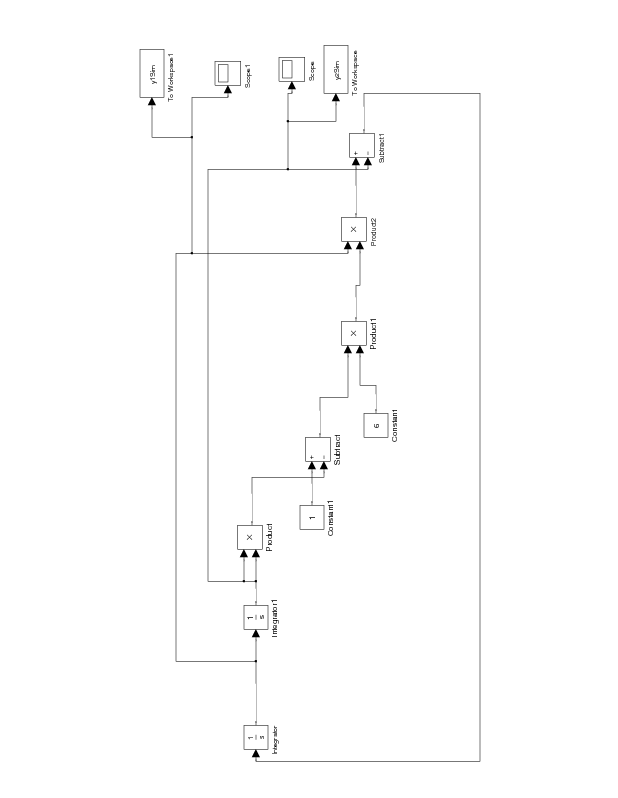
\includegraphics[width=\textwidth, angle=-90]{Prak1Aufg2Simulink.png}
            \caption{Van Der Pol Simulink}
            \label{pic:lorenzSimulink}
		\end{figure} 	
		
	\subsection{Iterationsgleichungen}	
	\subsubsection{Euler Verfahren}
	\begin{align}
		&z_{1_{n+1}} = z_{1_{n}} + h \cdot (6 \cdot (1-z_{2_{n}}^2) \cdot z_{1_{n}} - z_{2_{n}})\\
		&z_{2_{n+1}} = z_{2_n} + h * z_{1_n}
	\end{align}
	
	
	\subsubsection{Runge Kutta 2. Ordnung}
	Es gelte	
	\begin{align}
		g(t,y) = z \label{g}\\		
		f(y,z) = 6 \cdot (1-y^2) \cdot z - y \label{f}
	\end{align}
	Dann können wir durch einsetzen von (\ref{g}) und (\ref{f}) in Runge Kutta 2. Ordnung die Iterationsgleichungen erstellen:
	\begin{align}
		&y_{j+1}=y_j + \frac{h}{2} \cdot [g(t_j, y_j) + g(t_{j+1}, y_i h \cdot g(t_j, y_j))]\\
		&z_{j+1}=z_j + \frac{h}{2} \cdot [f(y_j, z_j) + f(y_{j+1}, z_j + h \cdot f(y_j, z_j))]
	\end{align} 
	
	
\subsection{Ergebnisse}
	\subsubsection{h=0.001}
		\begin{figure}[H]
			\centering	
			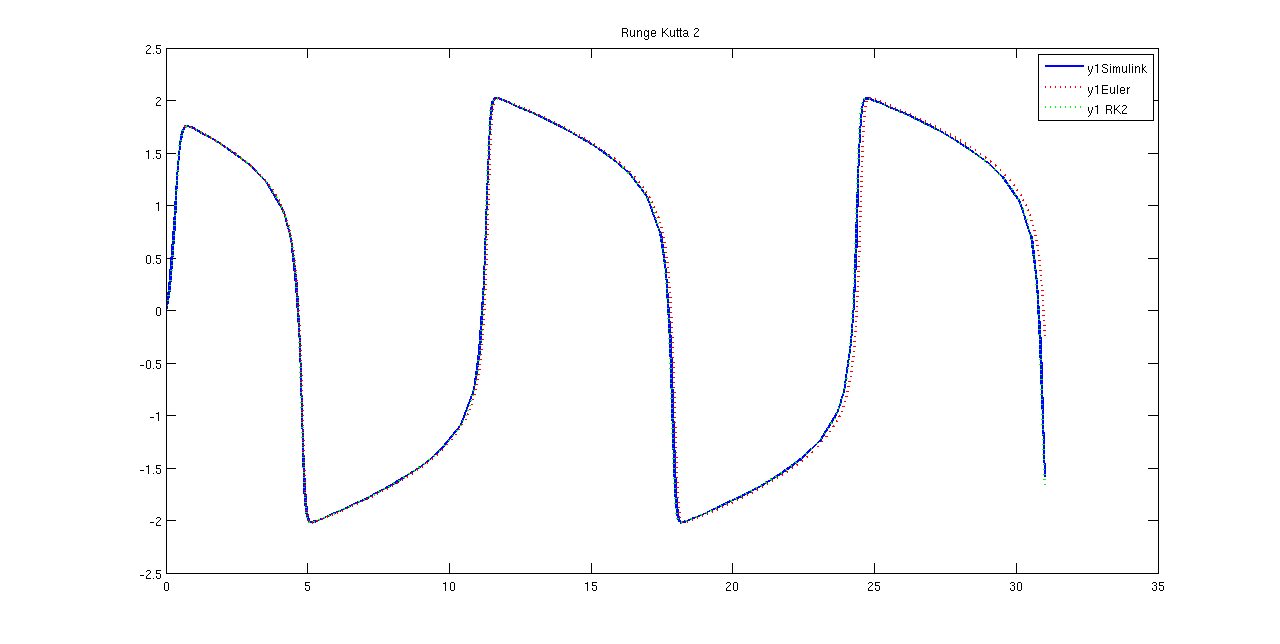
\includegraphics[width=\textwidth]{vanDerPolY10001.png}
            \caption{Van Der Pol DGL Y1 h=0.001}
            \label{pic:y2vdp0001}
		\end{figure} 
		
		\begin{figure}[H]
			\centering	
			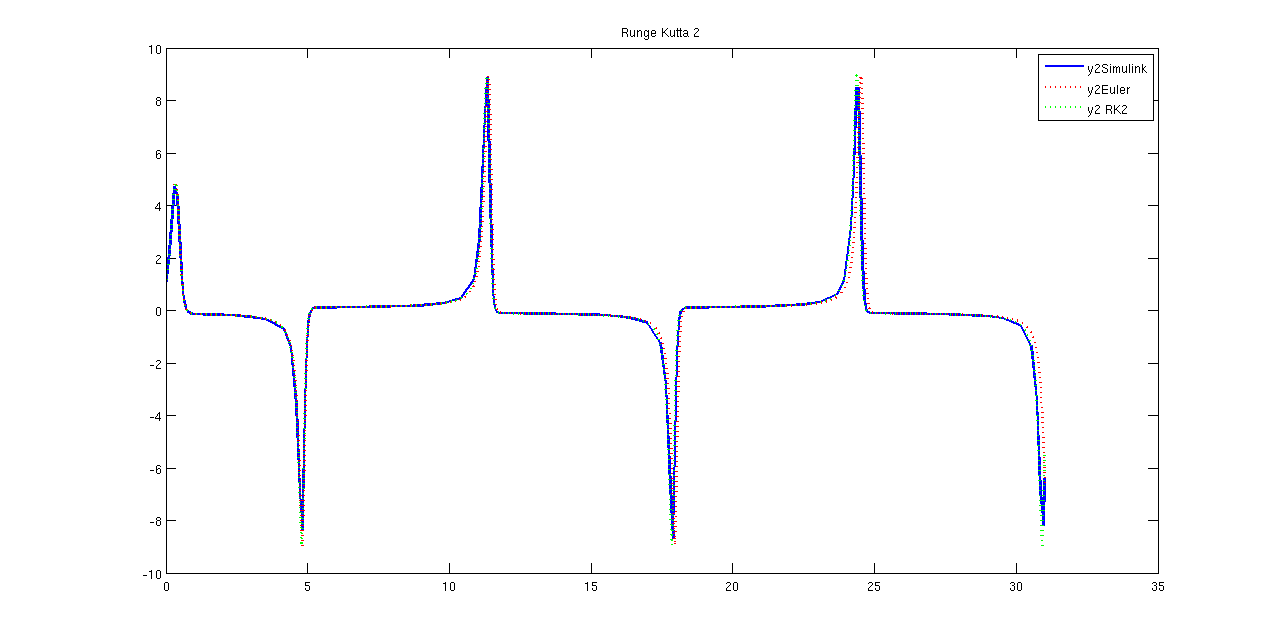
\includegraphics[width=\textwidth]{vanDerPolY20001.png}
            \caption{Van Der Pol DGL Y2 h=0.001}
            \label{pic:y2vdp0001}
		\end{figure}		
		
	Bei einer Schrittweite $h$ von $0.001$ ist zu erkennen das beide Approximationsverfahren (Expliziter Euler und Runge Kutta 2. Ordnung) mit der aus Simulink extrahierten Approximation (Dormand-Prince, Variable Step Size) übereinstimmen.
		
	\subsubsection{h=0.02}	
		\begin{figure}[H]
			\centering	
			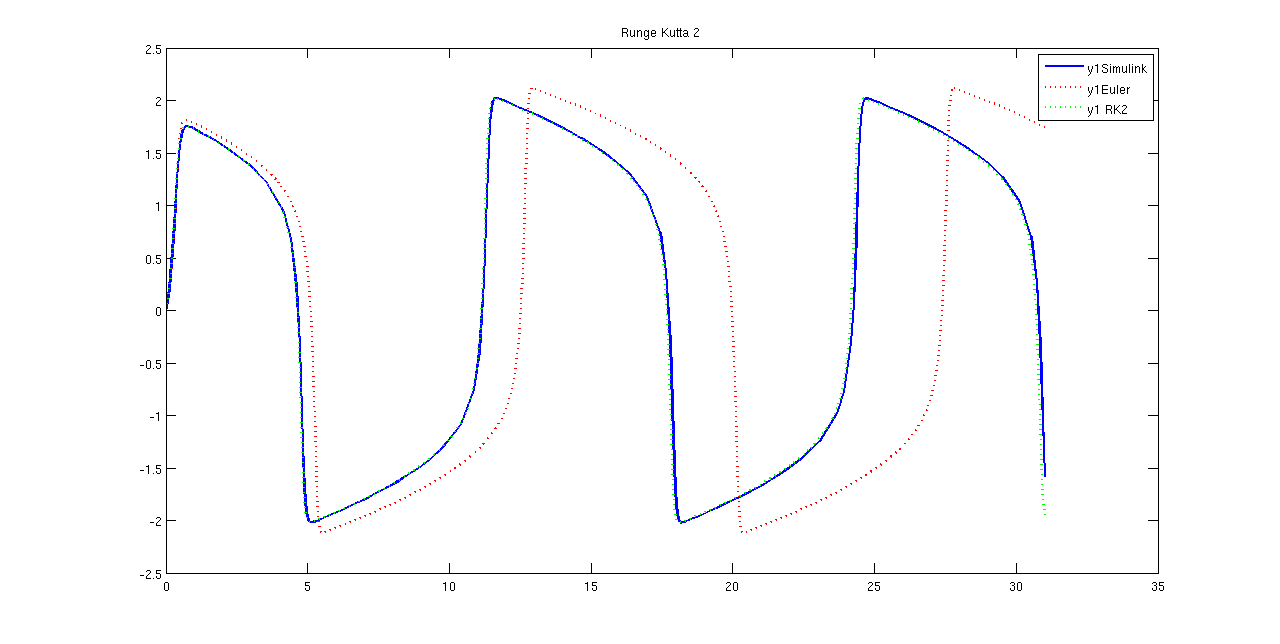
\includegraphics[width=\textwidth]{vanDerPolY102.png}
            \caption{Van Der Pol DGL Y1 h=0.02}
            \label{pic:y2vdp02}
		\end{figure} 
		
		\begin{figure}[H]
			\centering	
			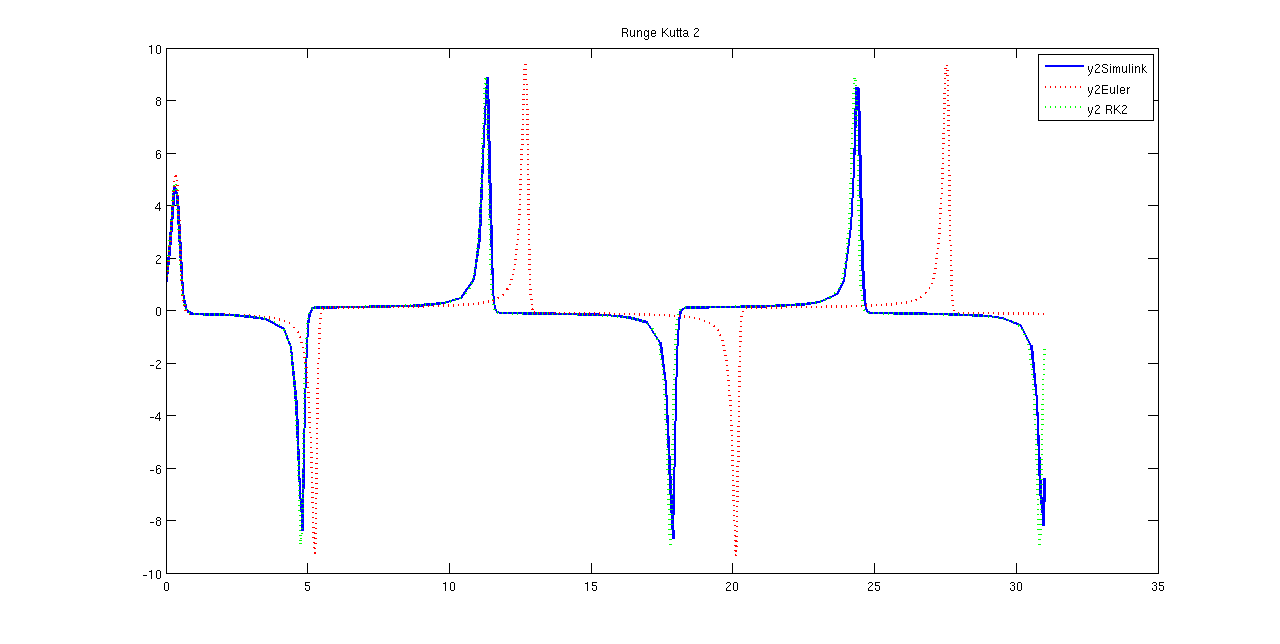
\includegraphics[width=\textwidth]{vanDerPolY202.png}
            \caption{Van Der Pol DGL Y2 h=0.02}
            \label{pic:y2vdp02}
		\end{figure}		
		
	Bei einer Schrittweite $h$ von $0.02$ ist zu erkennen das das simplere Approximationsverfahren (Expliziter Euler) deutlich von der aus Simulink extrahierten Approximation (Dormand-Prince, Variable Step Size) abweicht während das komplexere Verfahren (Runge Kutta 2. Ordnung) auch hier noch sehr dicht an Simulink liegt.
	
	\subsection{Matlab Programme}
	\lstinputlisting[tabsize=2, frame=single, label=vdp, caption={VanDerPol GDL}]{vdp.m}
	\lstinputlisting[tabsize=2, frame=single, label=vdpZeigen, caption={VanDerPol}]{vanDerPollZeigen.m}
		
		\section{Lorenz Attraktor}
		\subsection{Gleichung}
			\begin{align}
				&\dot{x}=-10 \cdot (x-y)\\
				&\dot{y}=(40-z)\cdot x-y\\
				&\dot{z}=x \cdot y - 2.67 \cdot z\\
				&x(0)=0.01\\
				&y(0)=0.01\\
				&z(0)=0.0
			\end{align}

		\subsection{Simulink}
		\begin{figure}[H]
			\centering	
			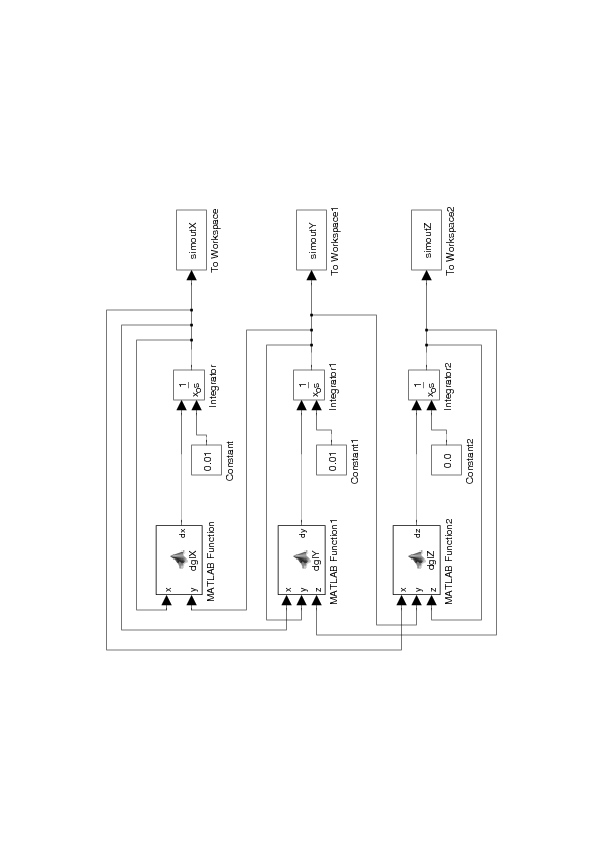
\includegraphics[width=\textwidth, angle=-90]{Prak1Aufg3Simulink.png}
            \caption{Lorenz Attraktor Simulink}
            \label{pic:lorenzSimulink}
		\end{figure} 
		
		
		\subsection{RK2}
		Gegeben
			\begin{align}
				&f(t,x)=-10 \cdot (x-y)\\
				&g(t,y)=(40-z)\cdot x-y\\
				&k(t,z)=x \cdot y - 2.67 \cdot z
			\end{align}
		So erhalten wir durch einsetzen in das Runge Kutta Verfahren 2. Ordnung folgende Iterationsgleichungen:
		
		\begin{align}
				&x_{j+1}=x_{j} + \frac{h}{2} \cdot (f(t_{j+1}, x_{j}) + f(t_{j+1}, h \cdot f(t_j, x_j)) )\\
				&y_{j+1}=y_{j} + \frac{h}{2} \cdot (g(t_{j+1}, y_{j}) + g(t_{j+1}, h \cdot g(t_j, y_j)) )\\
				&z_{j+1}=z_{j} + \frac{h}{2} \cdot (k(t_{j+1}, z_{j}) + k(t_{j+1}, h \cdot k(t_j, z_j)) )
		\end{align}
		
		\subsection{Ergebnisse}		
		Mit $h=0.002$, $t_{End} = 120$ und dem Parameter in der zweiten Gleichung auf $40$ ergeben sich folgende Funktionsplots für $x(t), z(t)$
		\begin{figure}[H]
			\centering	
			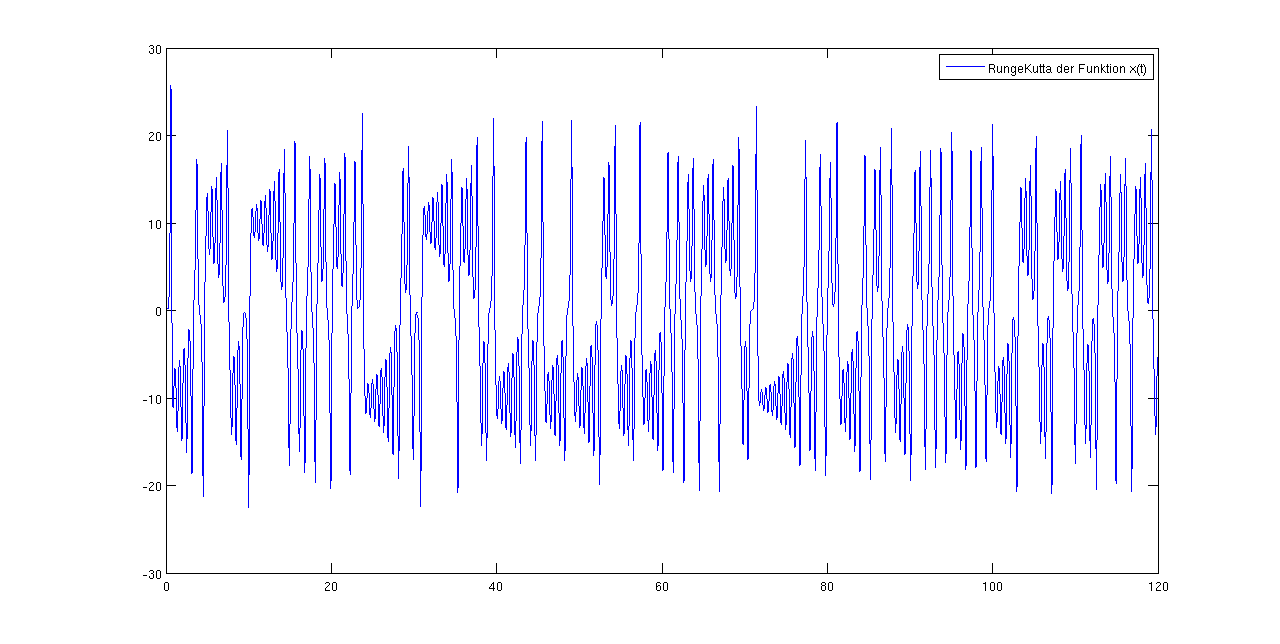
\includegraphics[width=\textwidth]{lorenzxt.png}
            \caption{Lorenz Attraktor x(t)}
            \label{pic:xt}
		\end{figure} 
		
		\begin{figure}[H]
			\centering	
			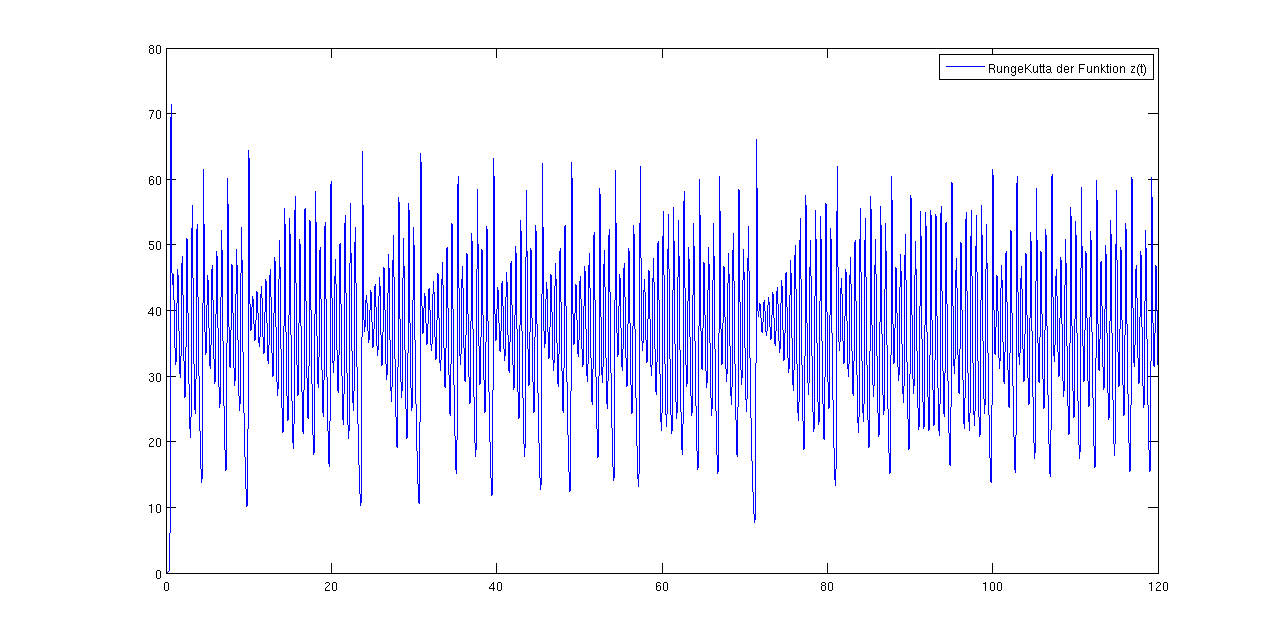
\includegraphics[width=\textwidth]{lorenzzt.png}
            \caption{Lorenz Attraktor z(t)}
            \label{pic:zt}
		\end{figure} 
		
		Wenn der konstante Parameter der zweiten Funktion auf $40.000000001$ geändert wird ergibt sich für $x(t)$ die folgende Veränderung. Es wird eine Verschiebung der Funktion erkennbar.  
		
		\begin{figure}[H]
			\centering	
			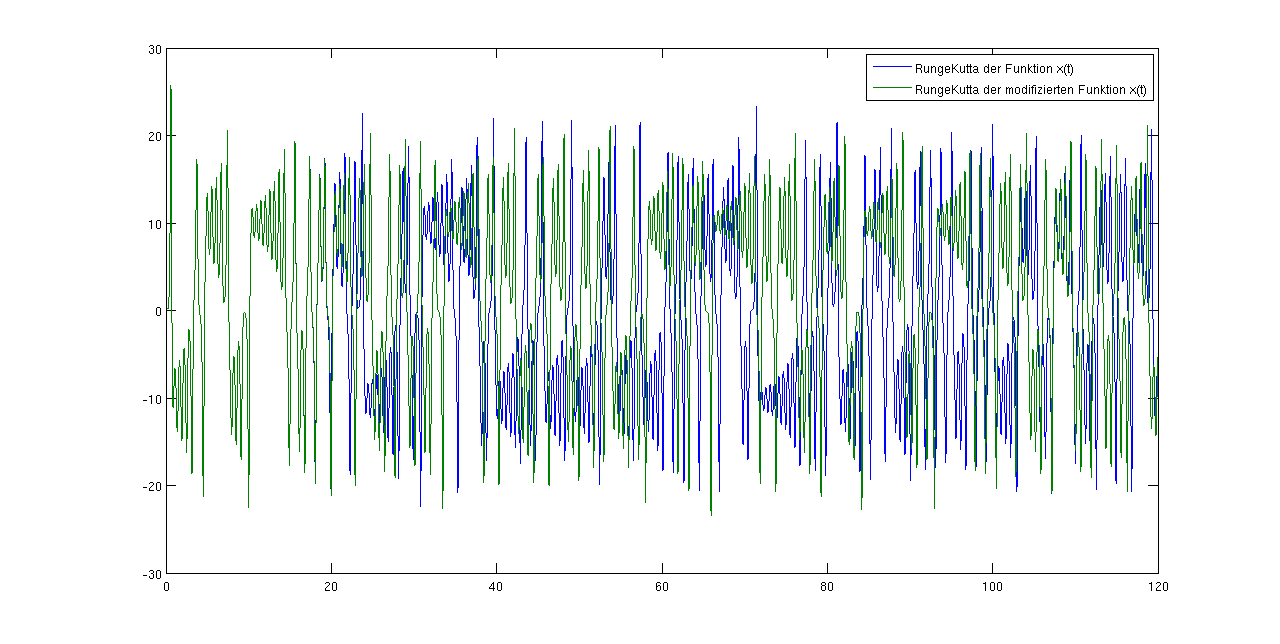
\includegraphics[width=\textwidth]{lorenzdif.png}
            \caption{Lorenz Attraktor Diff 40, 40.000000001}
            \label{pic:diff}
		\end{figure} 
		
		Die Auswertung der durch Simulink erzeugten Daten ergibt folgendes 3D Muster:
		\begin{figure}[H]
			\centering	
			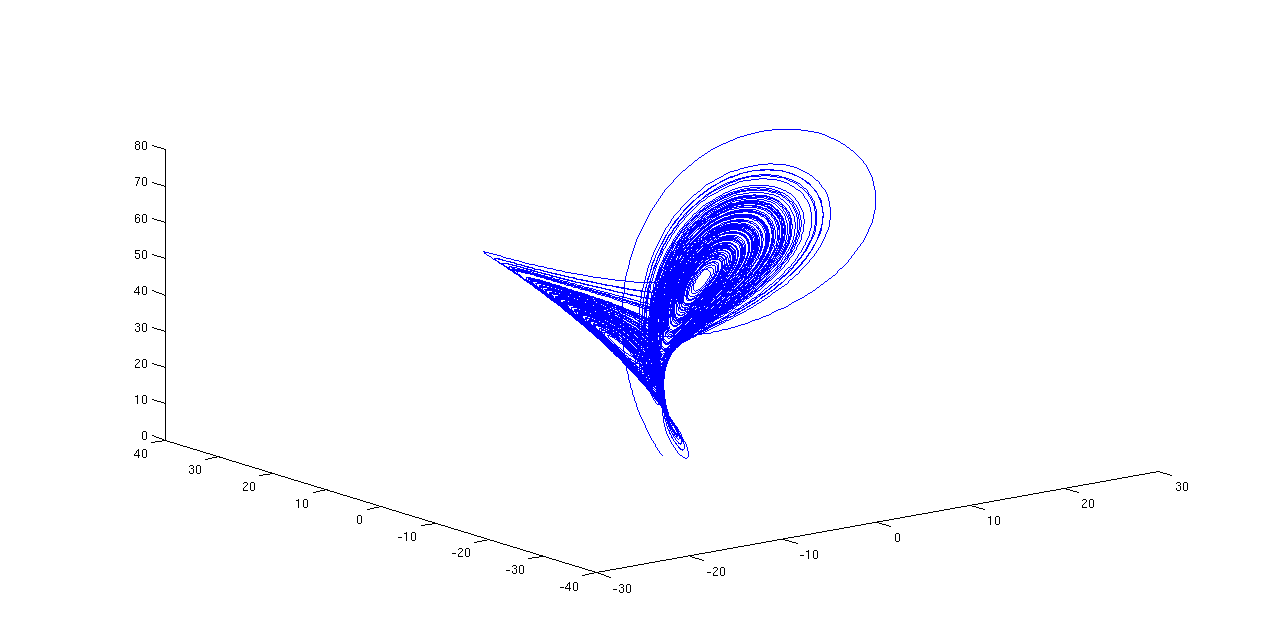
\includegraphics[width=\textwidth]{lorenz3d.png}
            \caption{Lorenz Attraktor 3D Plot}
            \label{pic:3dplot}
		\end{figure} 
		
\subsection{Matlab Programme}
	\lstinputlisting[tabsize=2, frame=single, caption={Lorenz Attraktor}]{dgls.m}
	\lstinputlisting[tabsize=2, frame=single, caption={Lorenz Attraktor mit verändertem Parameter}]{dglsUngenau.m}		
	\lstinputlisting[tabsize=2, frame=single, caption={Lorenz}]{LorenzAttraktor.m}		
		
		
	\section{Matlab Programme}	 \label{sec:matlab}
	\lstinputlisting[tabsize=2, frame=single, caption={Explizites Euler Verfahren}]{eulerE.m}
	\lstinputlisting[tabsize=2, frame=single, caption={Implizites Euler Verfahren}]{euler_impl.m}	
	\lstinputlisting[tabsize=2, frame=single, caption={Runge Kutta 2. Ordnung}]{rk2.m}		
		
\end{document}

